% This is LLNCS.DEM the demonstration file of
% the LaTeX macro package from Springer-Verlag
% for Lecture Notes in Computer Science,
% version 2.4 for LaTeX2e as of 16. April 2010
%
\documentclass{llncs}
\usepackage{graphicx}
%
\begin{document}
%
\title{Mobile Application Development with MELON}
%
\author{Justin Collins \and Rajive Bagrodia}
%
%%%% list of authors for the TOC (use if author list has to be modified)
\tocauthor{Justin Collins, Rajive Bagrodia}
%
\institute{University of California Los Angeles, Los Angeles CA, USA,\\
\email{\{collins, rajive\}@cs.ucla.edu}}

\maketitle

\begin{abstract}
Developing distributed applications for mobile ad hoc network continues to be challenging due to the dynamic and unpredictable nature of MANETs. MELON is a general purpose coordination language designed to provide flexible communication patterns for MANET applications while remaining lightweight. Based on a distributed shared message store, MELON abstracts network communication to an asynchronous exchange of persistent messages. MELON simplifies application development by supporting read-only and remove-only messages, bulk message retrieval, and per-host ordering of messages. In this paper, we review the MELON programming model, demonstrate its utility for writing MANET applications, and quantitatively compare it to traditional distributed computing paradigms in a MANET context. For a shared whiteboard application, we find MELON achieves 100\% message delivery with 95\% less latency than tuple spaces while also maintaining per-host message ordering.
\end{abstract}

\section{Introduction}

Tiny, powerful personal computers are quickly becoming ubiquitous. In the United States, 91\% of adults have cell phones, and 56\% of those are smartphones\cite{cellphones}. Among teens, 78\% have a cell phone, of which 37\% are a smartphone\cite{teenphones}. Add smartphones to the proliferation of tablets and laptops and the ability for consumers to form mobile ad hoc networks (MANETs) is quickly becoming possible. However, applications designed for these networks remain in short supply. Developing MANET applications presents a number of challenges with the primary difficulty being the unpredictably dynamic infrastructureless wireless network itself. Unlike wired networks, failures in MANETs are commonplace instead of exceptional. Nodes may join and leave the network at any time and the network topology is in constant flux. Networked applications must be aware of and handle the challenging nature of MANETs to be effective.

Several language, middleware, and library solutions to dealing with MANET communication have been proposed to assist in developing MANET applications. The majority of these proposals are based on traditional distributed computing paradigms\cite{mine}. Of these, publish/subscribe, remote procedure calls, and tuple spaces are commonly used. However, these communication paradigms were originally designed for stable, wired networks or even interprocedural communication on a single machine. While they have been adapted to MANETs, their original designs are limiting and not well-suited to the MANET environment\cite{collins2010quantitative}.

To address the need for a communication paradigm designed to operate in MANETs, we have proposed a new coordination language called MELON\cite{melon}. MELON provides a flexible, general-purpose communication abstraction which may be completely distributed. In addition to basic message exchange, MELON also implements bulk message retrieval, provides basic message access control, enforces per-host ordering of messages, and supports message streams.

In this paper we describe the MELON paradigm, compare implementing a shared whiteboard application with publish/subscribe, RPC, tuple spaces, and MELON, and finally compare the performance of each whiteboard implementation. We demonstrate MELON is well-suited for developing MANET applications, and while slower than publish/subscribe and RPC, it is the only paradigm to deliver 100\% of sent messages. MELON also delivered whiteboard messages with 95\% less latency and 60\% more in-order messages compared to tuple spaces.

Section \ref{sec:relatedwork} reviews the traditional paradigms used in this paper. In Section \ref{sec:design} we discuss the design of MELON, the operations it provides, and our prototype implementation. We compare a whiteboard implemented each paradigm in Section \ref{sec:wb} and then measure performance of each paradigm in Section \ref{sec:comparison} before presenting our conclusions in Section \ref{sec:conclusions}.

\section{Related Work}\label{sec:relatedwork}

This section offers a brief overview of the three paradigms we will compare with MELON. Further surveys of middleware, languages, and communication paradigms for MANET development can be found in \cite{mine} and \cite{mwtrends}.

The \textit{publish/subscribe} paradigm divides processes into publishers and subscribers. In topic-based publish/subscribe, publishers send messages tagged with a topic. Subscribers receive the messages by subscribing to one or more topics and specifying a callback to receive the publications asynchronously and separately from the main process thread. It is also possible to handle multiple incoming publications concurrently. Publish/subscribe does not guarantee any ordering of publications nor does it specify how to deliver messages if the subscribers is not available at the time of publication. In distributed publish/subscribe such as MANETs, it is generally not expected that publishers would persist and deliver messages at a later time via brokers\cite{psfaces}, although some implementations exist\cite{reds}. Managing an overlay network of brokers also adds considerable complexity.

\textit{Remote procedure calls} (RPC) is a distributed programming paradigm which disguises remote communication as local method calls. A host can ``export" an object to be accessed remotely. Remote hosts discover these remote objects by name or type and then invoke methods defined on the object. RPC is spatially coupled, since the remote object must be available in order to invoke the method. Arguments may be passed to the remote method and the return value of the method is returned to the local process. Since RPC implies code execution, failures during the remote calls can be dangerous\cite{distbook}.

Group RPC invokes the same method with the same arguments on all matching remote objects. In a MANET, group RPC must be performed asynchronously to be practical: the call may return multiple values but the client cannot rely on all remote hosts returning a value successfully. A timeout could be used instead, but a short timeout would cause unnecessarily lost messages, while a long timeout could cause long delays in the execution of the application.

\textit{Tuple spaces}, introduced in the Linda\cite{linda} coordination language, operate on a distributed shared memory space of ordered tuples. Tuples are sent using the \textbf{out} operation then retrieved by matching templates with \textbf{rd}, which copies the tuple, or \textbf{in}, which atomically removes the tuple from the tuple space. If multiple tuples match, one is chosen nondeterministically. Tuple spaces have strict semantics for \textbf{rd} and \textbf{in}: if a matching tuple exists, it \textit{must} be returned. \textbf{rd} and \textbf{in} are blocking operations, but typically nonblocking versions are available.

An issue particular to tuple spaces is the ``multiple read problem": nondestructively retrieving all matching tuples requires repeated \textbf{rd} operations, which may return any matching tuple. One solution is to use a mutex tuple to gain exclusive access to the tuple space, remove all matching tuples using \textbf{in}, replace the tuples, and then release the mutex. However, this approach prevents concurrent access and is dangerous in MANETs where the node with the mutex may disappear. Another solution uses a counter in each tuple and each process can request tuples by the counter value in order. Multiple processes producing tuples must coordinate to generate consistent counters. A third option proposed in \cite{mrdp} is to introduce a \textbf{copy-collect} operation which copies all matching tuples.

Several projects have adapted tuple spaces to MANETs, including L$^{2}$imbo\cite{limbo}, LIME\cite{lime}, TOTAM\cite{totam}, and EgoSpaces\cite{egospaces}. LIME, a popular implementation, relies on explicit join and leave operations to federate distributed tuple spaces. This is at odds with the frequently unexpected disconnections in MANETs. \cite{limerevisted} discusses the difficulties LIME encounters with tuple space semantics, including situations that can lead to livelocks. LIME II\cite{lime2}, Limone\cite{limone}, and CoreLIME\cite{corelime} are proposed to meet shortcomings in LIME.

\section{MELON Design}\label{sec:design}

MELON borrows the idea of a distributed shared message store from tuple spaces. The concept of shared message collections which may be safely manipulated by many processes fits well in a MANET context. To send a message, a process using MELON persists it in a globally shared ``store".  In practice these messages are stored on the client which outputs them in order maintain atomicity of removal without global state or locking. Messages are retrieved by matching against templates describing message content. This decoupling between sending and receiving is beneficial in a MANET context where maintaining connections between hosts can be challenging. With MELON and tuple spaces, disconnections do not cause lost messages or disrupt operations.

Aside from the shared message store, MELON departs significantly from typical tuple spaces in its operations and semantics. In a tuple space, any message may be read or removed by any process, and any matching message may be retrieved in any order. In contrast, MELON divides the messages into two pools: a remove-only pool, and a read-only pool. Remove-only messages can only be retrieved once and must be removed when retrieved. Read-only messages may never be explicitly removed, only be copied from the message store. Matching messages are returned in FIFO order per host, matching the reliable FIFO-ordered multicast semantics in \cite{distbook}.

MELON contains some additional minor differences from tuple spaces. First, messages are not required by the paradigm to be tuples, but may be implemented as any structure which can be matched by a template (e.g., messages could be unordered tuples with named values instead). Secondly, MELON explicitly acknowledges the storage limitations of mobile devices. In any communication paradigm which persists messages, there is a limitation to how many messages may be stored. MELON attempts to mitigate this limitation by allowing messages to be automatically garbage collected. The alternatives are to not store new messages or to allow applications to exhaust available memory.

A last deviation from tuple spaces is the removal of strict semantics for returning messages. In tuple spaces, the semantics stipulate that if a matching message exists, it must be returned for a retrieval operation. In the reality of MANETs, this semantic cannot be met, so in MELON all retrieval operations are limited to best-effort.

These differences were introduced in MELON to both relieve the application developer of certain responsibilities and to allow the paradigm to operate well in a MANET. For example, read-only messages prevent a badly-behaved process from removing important messages meant to be read by many processes, and FIFO ordering is especially convenient in applications where most messages are generated by a single host and the ordering is important, such as news feeds or streaming video. MELON is also deliberately designed to avoid any global state and enable completely distributed implementations.

\subsection{MELON Operations}\label{melon}

Processes in MELON communicate by storing messages to a distributed shared message store and retrieving the messages based on templates. In this paper, we assume messages consist of an ordered list of typed values. However, as noted above, MELON does not limit how messages might be constructed. A message template is similar to a message, except it may contain both values and types. For example, a message containing \texttt{[1, "hello"]} could be matched by a template containing \texttt{[1, String]} or \texttt{[Integer, "hello"]} or \texttt{[Integer, String]}. A type will also match any subtypes.

Operations are split into read-only (\textbf{write}/\textbf{read}/\textbf{read\_all}) and take-only (\textbf{store}/\textbf{take}/\textbf{take\_all}) operations. Each operation is represented here as a separate function call. \textbf{store} and \textbf{write} operations return null values as soon as the saved message is available in the message store (essentially immediately). \textbf{take} and \textbf{read} operations block by default until a matching message is returned, but may be set to nonblocking on a per-call basis. If a nonblocking operation finds no matching messages, an empty set is returned.

\begin{table}
\centering
\caption{MELON Operations}
\begin{tabular}{|c|c|c|}
\hline
\textbf{Operation} & \textbf{Return Type} & \textbf{Action} \\ \hline
\textbf{store}(\textit{message}) & \textit{null} & Store removable message \\ \hline
\textbf{write}(\textit{message}) & \textit{null} & Store read-only message \\ \hline
\textbf{take}(\textit{template}, \textit{[block = true]}) & \textit{message} or \textit{null} & Remove and return message \\ \hline
\textbf{read}(\textit{template}, \textit{[block = true]}) & \textit{message} or \textit{null} & Copy and return read-only message \\ \hline
\textbf{take\_all}(\textit{template}, \textit{[block = true]}) & \textit{array} & Bulk remove messages \\ \hline
\textbf{read\_all}(\textit{template}, \textit{[block = true]}) & \textit{array} & Bulk copy read-only messages \\ \hline
\end{tabular}
\end{table}

When called, \textbf{store} saves a copy of the message in the message store. Messages saved with \textbf{store} may only be retrieved with a \textbf{take} or \textbf{take\_all} operation.

The \textbf{write} operation also stores a single message in the message store, but the message may only be copied from the storage space with a \textbf{read} operation, never explicitly removed. Messages stored with either operation may be automatically garbage collected.

A \textbf{take} operation accepts a message template as the first argument and an optional boolean indicating blocking or nonblocking for the second argument. The message template is matched against available messages in the message store which were added with a \textbf{store} operation. If a matching message is found, it will be removed from the message store and returned. Once a message has been returned by a \textbf{take} operation, it may not be returned by a subsequent operation in any process.

The \textbf{read} operation accepts the same arguments but will only return messages stored with a \textbf{write} operation which have not already been read by the current process. If a message matching the given message template is available, it will be copied and returned, but not removed from the message store. Once a message has been returned to a process, the message is considered to have been read by that process and will not be returned by any subsequent \textbf{read} or \textbf{read\_all} operations in that process. A message may be \textbf{read} by any number of processes, but only once per process.

\begin{table}
\centering
\caption{Read from multiple processes}
\begin{tabular}{|c|c|c|} \hline
\textbf{Process A} & \textbf{Process B} & \textbf{Process C} \\ \hline
\texttt{write([1, "hello"])} & \texttt{m = read([Integer, String])} & \texttt{m = read([Integer, String])} \\ \hline
\end{tabular}
\label{fig:readprocesses}
\end{table}

Table \ref{fig:readprocesses} illustrates one process writing a single message containing the integer \texttt{1} and the string \texttt{"hello"}. Processes B and C each perform a \textbf{read} operation with the template which matches the message stored by process A. Since \textbf{read} does not modify the storage space, the value of \textit{m} for both process B and C will be a copy of the message \texttt{[1, "hello"]} from process A.

The \textbf{take\_all} and \textbf{read\_all} operations are used to retrieve a group of matching messages instead of a single message. Otherwise, the semantics match \textbf{take} and \textbf{read}: \textbf{take\_all} can only remove messages from \textbf{store} operations, and \textbf{read\_all} only returns unread messages from \textbf{write} operations. Table \ref{fig:newsreader} demonstrates a use of \textbf{read\_all}. One or more processes generate news messages containing a news category and headline. To ensure all interested parties can read the news, the server uses \textbf{write} to disallow a reader from removing a news item and preventing other readers from reading it. Any number of processes can consume the news as readers. The \texttt{fetch} method in Table \ref{fig:readprocesses} uses \textbf{read\_all} to return all news items in a given category. Repeated calls to \texttt{fetch} will only return news items not previously read.

\begin{table}
\centering
\caption{News server and reader}
\begin{tabular}{|c|c|} \hline
\textbf{News Server} & \textbf{News Reader} \\ \hline
\begin{minipage}{2.45in}
\begin{verbatim}

def report(category, headline)
   write [category, headline]
end 
\end{verbatim}
\end{minipage}
&
\begin{minipage}{2.5in}
\begin{verbatim}

def fetch(category)
   return read_all([category, String])
end
\end{verbatim}
\end{minipage}
\\ \hline
\end{tabular}
\label{fig:newsreader}
\end{table}

By default, all retrieval operations will block the application until at least one matching message is found. The operations can also be performed in nonblocking mode, in which case \textbf{take} and \textbf{read} return null when no matching message is found, while \textbf{take\_all} and \textbf{read\_all} return empty collections.
   
\subsection{MELON Implementation}\label{sec:implementation}

\begin{figure}
\centering
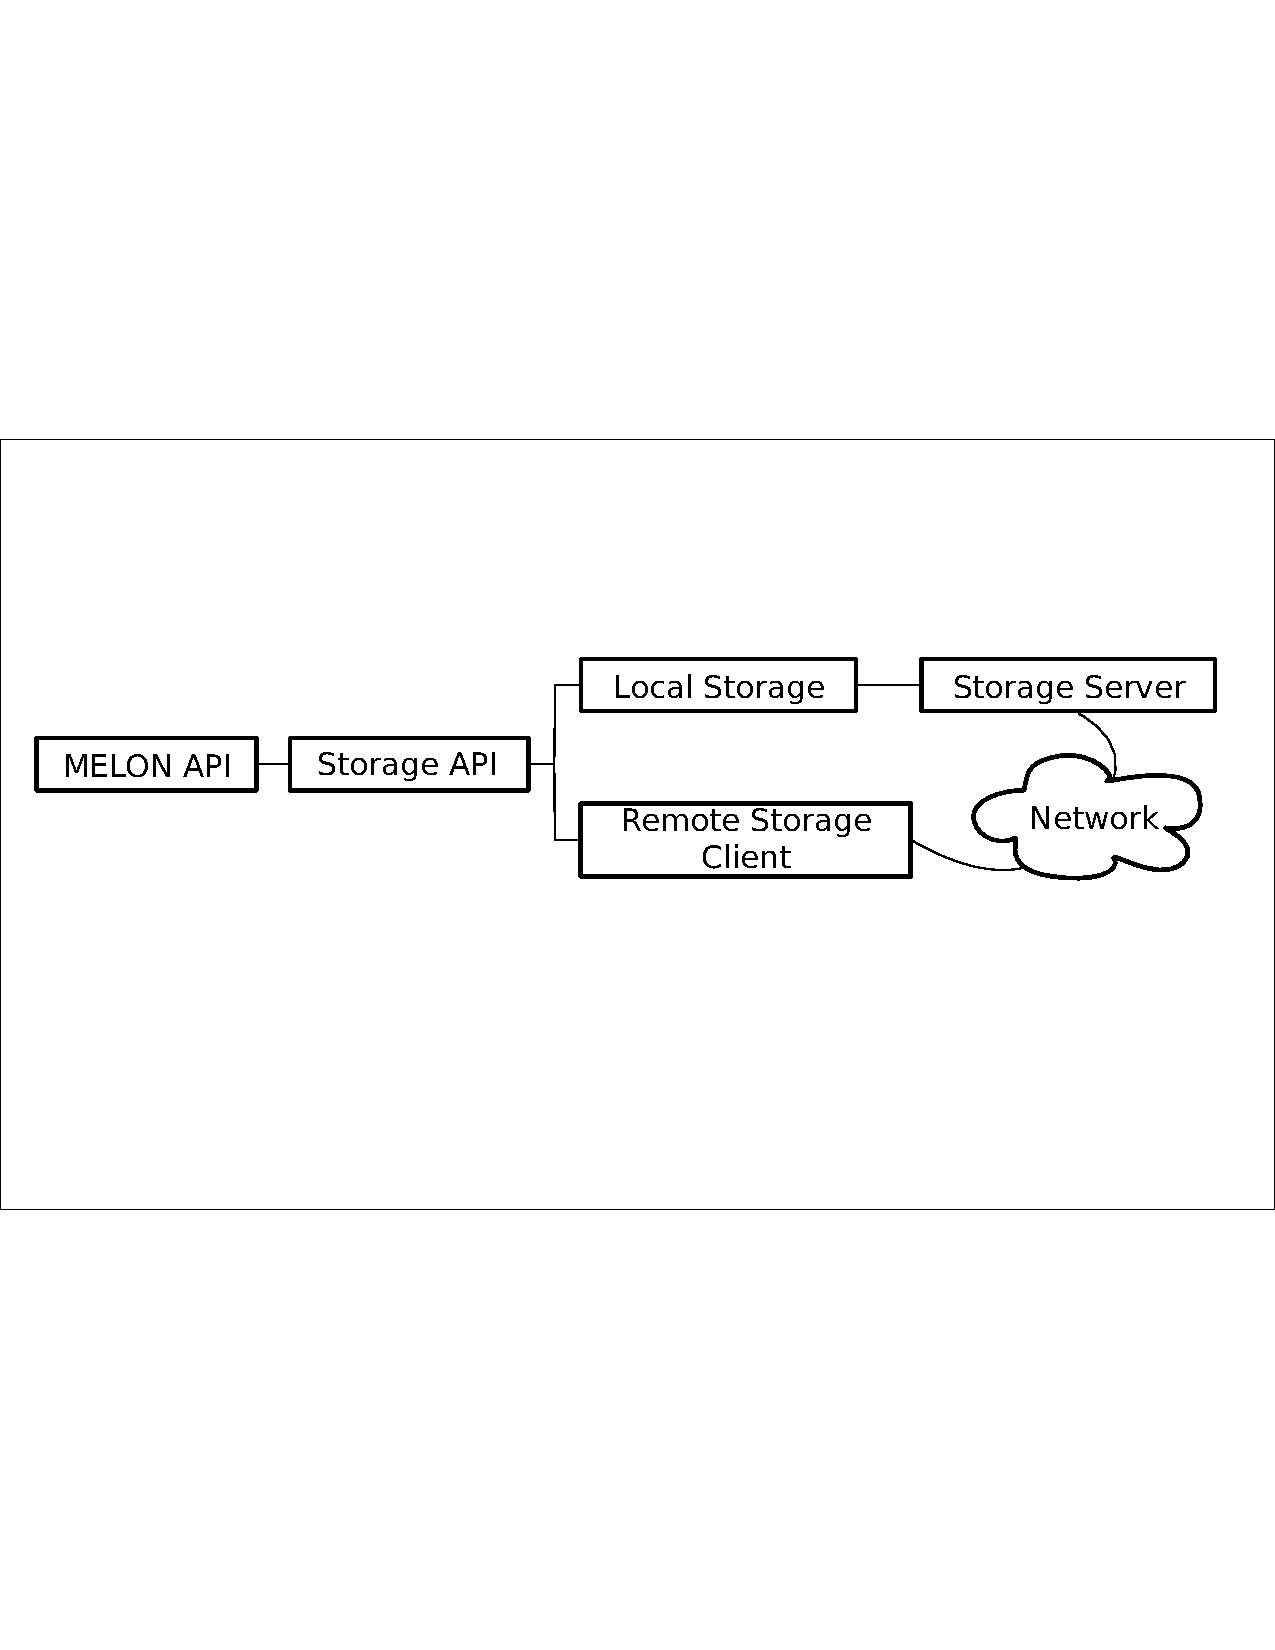
\includegraphics[scale = .45, clip, trim = 10px 350px 10px 312px]{figures/paradigm_arch.pdf}
\caption{Paradigm Architecture}
\label{fig:architecture}
\end{figure}

We developed a prototype implementation of MELON to validate our design and obtain empirical performance data. The architecture illustrated in Figure \ref{fig:architecture} is split into five parts. The MELON API is the only interface exposed to the application and provides the six operations described in Section \ref{sec:design}. The MELON API interacts with the distributed message storage through the storage API, which provides the same interface for both local and remote storage. The storage server proves a network interface to a local storage space and accepts connections made through the remote storage stub.

Local storage is implemented as two dynamic arrays, one for \textbf{write} / \textbf{read} messages and the other for \textbf{store}/\textbf{take} messages. For atomic updates, the \textbf{write} / \textbf{read} array uses a readers/writer lock to allow multiple \textbf{read} operations to access the array concurrently, but locks the array for \textbf{write} operations. The \textbf{store}/\textbf{take} array does not permit concurrent operations, as \textbf{store} and \textbf{take} modify the store. The two arrays may be accessed and modified independently. Searching for matching messages is a linear operation in the prototype implementation. Performance of local operations is explored in \cite{melon}.

Network communication is handled by ZeroMQ\cite{hintjens2013zeromq}, a high performance networking library. For the prototype, the networking was intentionally kept simple. For example, a \textbf{read} request queries remote hosts in random order and stops when a matching result is returned. This could possibly be improved using multicast, but it would complicate the implementation by requiring the client to handle multiple asynchronous responses, select one, request the actual message, and handle failure scenarios if the matching message cannot be returned. We traded potential performance gains for simplicity.

For \textbf{read} and \textbf{read\_all} operations, it is necessary to track which messages have been read. Each process maintains its own list of read messages, which it sends with each \textbf{read} request. We use a compact sparse bit set to track message IDs and transfer this information efficiently with an average overhead of $<2$ bits per ID.

\section{Shared Whiteboard Example}\label{sec:wb}

A shared whiteboard is a digital document which may be edited and viewed by multiple users concurrently and is commonly given as an example of an application well-suited to MANETs\cite{wb6}. Shared whiteboards are distributed, real-time, and interactive, which presents some interesting characteristics. Many participants must have access to update the whiteboard, but ordering of changes is very important to maintain a consistent document. Changes should be propagated quickly and reliably so that each user is working with the latest document without missing any updates.

We have implemented a shared whiteboard in MELON along with canonical versions of publish/subscribe, RPC, and tuple spaces using JRuby (a Java implementation of the Ruby language) to compare their features and performance. The programs share common code related to the actual whiteboard itself, which is implemented in the \texttt{Whiteboard} class. Changes to the shared whiteboard are encapsulated in a \texttt{Figure} object. Each version implements an \texttt{add\_local\_figure} method to be called when the user modifies the shared whiteboard. The MELON and tuple space versions also implement an \texttt{add\_remote\_figures} method which is used to retrieve updates from remote nodes.

\subsection{Publish/Subscribe}

The publish/subscribe whiteboard in Table \ref{fig:pswb} sets up a subscription to the ``whiteboard" topic and a callback to add remotely published figures to the whiteboard. This allows the whiteboard to receive updates at any time in a separate thread, which is precisely what would be desired. To output a new figure, the whiteboard simply publishes the figure to the ``whiteboard" topic.

\begin{table}
\centering
\begin{tabular}{c c}
\begin{minipage}{2.75in}
\caption{Publish/Subscribe Whiteboard}\label{fig:pswb}
\begin{verbatim}
require "ps"
require "whiteboard"

class PSWhiteboard < Whiteboard
  def initialize
    @ps = PS.new
    
    @ps.subscribe("whiteboard") do |figure|
      add_figure(figure)
    end
  end

  def add_local_figure(figure)
    @ps.publish("whiteboard", figure)
  end
end
\end{verbatim}
\end{minipage}
&
\begin{minipage}{2.5in}
\caption{RPC Whiteboard}\label{fig:rpcwb}
\begin{verbatim}
require "rpc"
require "whiteboard"

class RPCWhiteboard < Whiteboard
  def initialize
    @rpc = RPC.new
    @rpc.export(self)
  end

  def add_local_figure(figure)
    wbs = @rpc.find_all("RPCWhiteboard")
    wbs.add_figure(figure)
  end
end


\end{verbatim}
\end{minipage}
\end{tabular}
\end{table}


\subsection{RPC}

A shared whiteboard implementation using RPC is listed in Table 5. When the whiteboard is initialized, it exports itself as a remote object. Remotes hosts can then remotely invoke \texttt{add\_figure}. Like publish/subscribe, this allows the whiteboard to accept remote figures asynchronously from the main process thread and is a natural feature of RPC. Distribution of remote figures is performed by first finding all remote instances of \texttt{RPCWhiteboard}, then invoking the \texttt{add\_figure} method (defined on the parent class) directly, passing in the new figure as an argument. Since group RPC is asynchronous, it is possible that a call might complete before a prior call.

\subsection{Tuple Spaces}

Table \ref{fig:tswb} shows the tuple space version, which is very similar to MELON. To send an update, it outputs a tuple containing just the new figure. Unlike MELON, a misbehaving or misconfigured client could remove the messages from the tuple space, disrupting the shared whiteboard communication. Retrieval of remote messages uses a \textbf{bulk\_rd} operation to read all messages containing a figure. To continuously retrieve messages asynchronously, this method can be called inside a loop in a separate thread. Once a group of figures is retrieved, each individual figure is added to the local whiteboard. 

As discussed in Section \ref{sec:relatedwork}, \textbf{copy-collect} may be used to solve the ``multiple read problem''. We have implemented this as the \textbf{bulk\_rd} operation. However, this does not solve what might be termed the ``multiple multiple read problem": since our tuple space is not static, reading all matching tuples once is not sufficient. We need to be able to perform multiple \textbf{bulk\_rd}s to add all figures the whiteboard. Without \textit{a priori} knowledge of remote hosts in the system, the only option which allows concurrent access to the tuple space is to read \textit{all} matching tuples. Naturally, this becomes considerably expensive as the number of tuples grows large.

\begin{table}
\centering
\begin{tabular}{c c}
\begin{minipage}{2.75in}
\caption{MELON Whiteboard}\label{fig:mwb}
\begin{verbatim}
require "melon"
require "whiteboard"

class MelonWhiteboard < Whiteboard
  def initialize
    @melon = Melon.new
  end
  
  def add_local_figure(figure)
    @melon.write([Figure])
  end

  def add_remote_figures
  	 # Returns only unread figures
  	 # in per-host order
    figures = @melon.read_all([Figure])

    figures.each do |figure|
      add_figure(figure[0])
    end
  end
end
\end{verbatim}
\end{minipage}
&
\begin{minipage}{2.5in}
\caption{Tuple Space Whiteboard}\label{fig:tswb}
\begin{verbatim}
require "tuplespace"
require "whiteboard"

class TSWhiteboard < Whiteboard
  def initialize
    @ts = Tuplespace.new
  end

  def add_local_figure(figure)
    @ts.out([Figure])
  end

  def add_remote_figures
  	 # Returns ALL figures
  	 # in arbitrary order
    figures = @ts.bulk_rd([Figure])

    figures.each do |figure|
      add_figure(figure[0])
    end
  end
end	
\end{verbatim}
\end{minipage}
\end{tabular}
\end{table}

\subsection{MELON}

The MELON whiteboard in Table \ref{fig:mwb} writes out each figure in a tuple containing just the new figure. It uses the \textbf{write} operation since every remote node needs to read the figures. To retrieve remote figures, MELON uses \textbf{read\_all} to nondestructively read all messages containing a \texttt{Figure}. Like tuple spaces, the \texttt{add\_remote\_figures} method should be called in a separate thread to provide asynchronous updates. Unlike tuple spaces, MELON's \textbf{read\_all} operation only retrieves unread messages, eliminating the ``multiple multiple read" problem.

MELON directly provides three features which are helpful to the whiteboard application: persistent messages, reading only unread messages, and returning messages in a per-host FIFO ordering. Message persistence is crucial in MANET applications, where communication with remote nodes is often disrupted and delayed. For a shared whiteboard, every message must be delivered to keep the document synchronized between users. By managing read versus unread messages, MELON easily allows the whiteboard to efficiently fetch only newly-added figures. Finally, MELON guarantees the updates from each host will be retrieved in the order the host initiated them.

\subsection{Summary}

All four implementations of the whiteboard have been kept as simple and similar as possible in order to highlight the differences between the paradigms. However, while MELON appears to be as simple to use as the other paradigms, it provides more functionality and guarantees.

Publish/subscribe and RPC are push-based paradigms and allow messages to be received asynchronously by default. However, they do not provide message persistence in their canonical forms. While publish/subscribe is a multicast paradigm by default, RPC must be adapted to perform group communication. Also, RPC must explicitly discover remote objects before invoking remote methods. In both paradigms figures are sent and received singly, although multiple messages may be received concurrently.

Tuple spaces and MELON are pull-based paradigms which provide message persistence. Both tuple spaces and MELON require applications to explicitly use a separate thread to receive messages asynchronously. Tuple spaces do not provide a method to nondestructively read a subset of matching tuples, while MELON does. MELON is also the only paradigm to provide some ordering of messages by definition. Both paradigms allow bulk retrieval of messages, although tuple spaces require an extension to the canonical paradigm. This extension is necessary to allow nondestructive reads of multiple matching tuples and avoid the ``multiple read" problem.

\section{Quantitative Comparison}\label{sec:comparison}

For these experiments, we implemented the shared whiteboards as described in Section \ref{sec:wb} in the four paradigms using the same codebases as in \cite{melon}. To make the comparison as fair as possible, each paradigm shares a considerable amount of common code and utilizes ZeroMQ for network communications.The tuple space implementation uses the LighTS\cite{lights} local tuple space library from LIME.

To evaluate the implementations in a MANET environment, we used EXata\cite{exata} to provide high-fidelity wireless models and precisely repeatable scenarios while allowing us to run real applications. Our scenario uses 50 nodes with 802.11b radios using AODV moving with random waypoint with a maximum speed of 5m/s in a 500x500 meter area. The two-ray path loss model is used. To measure how the implementations fared in turbulent network conditions, we performed the experiments with increasing levels of packet loss from 1\% to 30\% as measured by the \textit{ping} command. We used an experiment coordination framework written in MELON itself to manage the applications, running EXata, and collating results.

In our scenario, six real nodes are running the whiteboard application, the rest are simulated and function only as intermediate nodes. For each experiment, each of the six nodes sends 50 whiteboard updates with pauses of 5-10 seconds. This roughly models each user updating their whiteboard at a brisk pace for 4-8 minutes.

\subsection{Results}

For each implementation, we measured lost messages, messages received out of order, and the message latency. For out-of-order messages, we divided it into two metrics: host out-of-order and global out-of-order. Host out-of-order messages are messages from a single host which are not received in the order sent. Global out-of-order messages are those received before their preceding message. For example, node A receives a message \textit{m}$_{1}$ from node B, then sends \textit{m}$_{2}$. If node C receives \textit{m}$_{2}$ prior to \textit{m}$_{1}$, \textit{m}$_{2}$ will be considered globally out of order.

As guaranteed by the paradigm, MELON maintains host ordering in all scenarios while publish/subscribe and RPC do not. For global message ordering, MELON outperforms tuples spaces by 67\% and remains within 15\% of RPC performance until packet loss reaches 30\%. However, this is because MELON continues to achieve 100\% message delivery while RPC drops nearly 12\% of messages when the network conditions are poor. Reliability does decrease speed, but MELON experiences 95\% less latency than tuple spaces while remaining within 3 seconds of RPC in the worst case. While we would like speed, reliability, and perfect ordering of messages for a shared whiteboard, it is better to have the document be eventually consistent than to lose information.

\begin{figure}[ht]
\centering
\begin{minipage}[b]{0.48\linewidth}
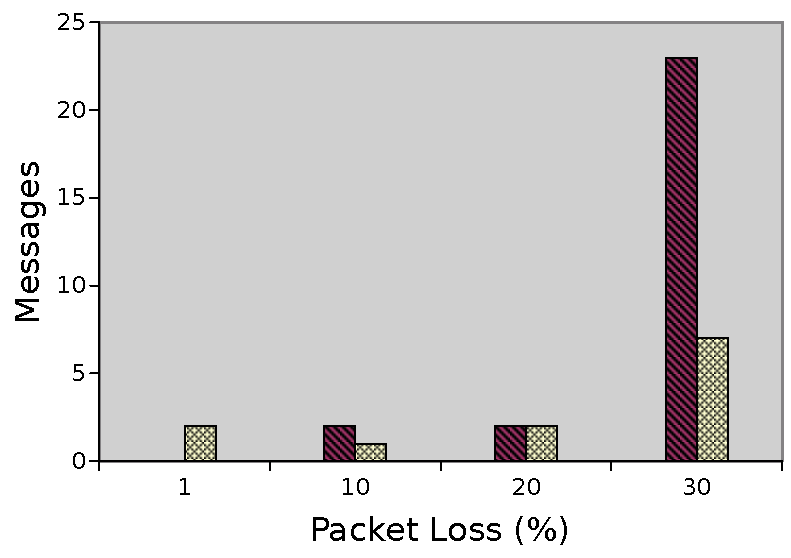
\includegraphics[width = \textwidth]{figures/hooo.pdf}
\caption{Host Out-of-Order Messages}
\label{fig:hooo}
\end{minipage}
\quad
\begin{minipage}[b]{0.48\linewidth}
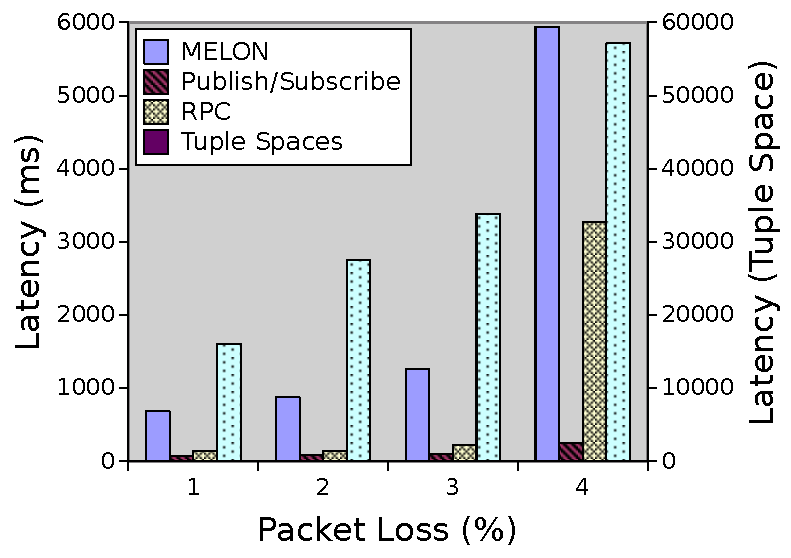
\includegraphics[width = \textwidth]{figures/latency.pdf}
\caption{Message Latency}
\label{fig:latency}
\end{minipage}
\end{figure}

In our experiments, messages from a single host were generally delivered in the order they were sent as shown in Figure \ref{fig:hooo}. For MELON and tuple spaces, no messages were delivered out of order. Note for tuple spaces this is an accident of the implementation, whereas in MELON it is guaranteed. In LighTS, tuples are sequentially stored locally in an array in the order they are output, then returned in that same order when they are matched. Tuple spaces in general do not return matched messages in any particular order.

Asynchronous group RPC is used in this application. If one call is delayed, it is possible a subsequent call will complete before a prior one, which is why RPC delivers a small number of messages out of order. Publish/subscribe is fully asynchronous and incoming publications can be processed concurrently. However, even in the worst case publish/subscribe delivers 97.8\% of the messages from a host in FIFO order. Like tuple spaces this is the result of the implementation: the RPC and publish/subscribe paradigms make no promises about the ordering of messages.

Unlike per-host ordering, many messages were delivered out of order from a global perspective as can be seen in Figure \ref{fig:gooo}. This is entirely expected, since none of the paradigms provide a global ordering. Enforcing a global ordering in an unreliable network is not feasible, since nodes may become unavailable at any time while continuing to output messages. However, the global ordering remains important for a shared whiteboard.

Our results show publish/subscribe performs the best for this metric. Indeed, ordering is largely dependent on deliveries completing quickly before later messages overtake them. As shown in Figure \ref{fig:latency}, publish/subscribe is an extremely quick method for delivering messages, so it excels in ordering as well. Conversely, tuple spaces fare the worst, delivering 67\% of messages out of order. Again, because tuple spaces provide no way of controlling which matches messages are returned or in what order, the whiteboard implementation must transfer large amounts of tuples in order to nondestructively read all matching messages. This is extremely slow, as reflected in Figure \ref{fig:latency}.

MELON and RPC provide about the same global ordering, although MELON is more affected when the network conditions worsen. This is likely due to MELON's reliable message delivery (Figure \ref{fig:delivery}), as messages may be delayed significantly by broken routes or network partitioning. In contrast, losing messages improves ordering since a message not delivered cannot be out of order. MELON is the only paradigm to demonstrate 100\% message delivery. Tuple spaces are expected to be reliable, but this application requires delivery of large numbers of messages. Since the median latency for tuple spaces reached a full minute, the experiment completed before all messages arrived.


\begin{figure}[ht]
\centering
\begin{minipage}[b]{0.48\linewidth}
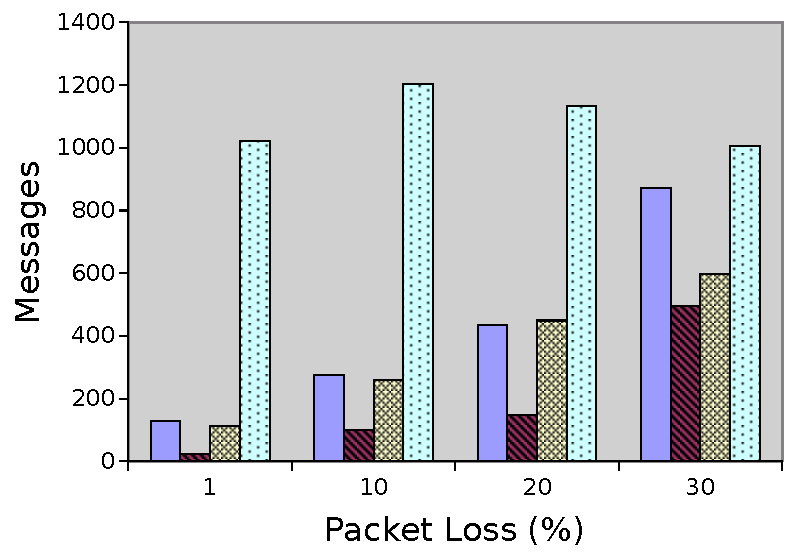
\includegraphics[width = \textwidth]{figures/gooo.pdf}
\caption{Global Out-of-Order Messages}
\label{fig:gooo}
\end{minipage}
\quad
\begin{minipage}[b]{0.48\linewidth}
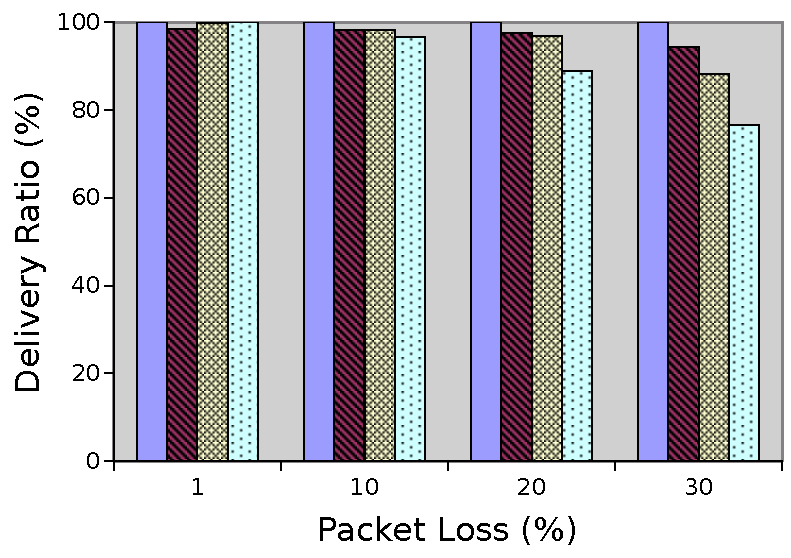
\includegraphics[width = \textwidth]{figures/delivery.pdf}
\caption{Delivery Rates}
\label{fig:delivery}
\end{minipage}
\end{figure}

While low delivery rates for publish/subscribe have been observed previously\cite{collins2010quantitative}, here it performs well in the lossy environment due to quick delivery rates, but still dropped 1.4\% of messages when the network connectivity was good. RPC never achieves 100\% delivery rates and declines as the network degrades. In group RPC, clients cannot be aware of how many receivers may be available and therefore does not attempt to retry calls after timeouts. Synchronous RPC would block the process until the message is delivered, but deliveries would be considerably delayed which is unacceptable for this application.

Median time between sending and receiving a message is reported in Figure \ref{fig:latency}. Since tuple spaces are so much slower, the results are aligned with the right-hand y-axis which is an order of magnitude higher. Publish/subscribe was extremely quick, as it requires no message confirmations nor active discovery of remote hosts. RPC was also quite fast until it was disrupted by the 30\% packet loss.

Logically, delivery rates and latency are directly related. With reliable delivery some messages may be very late, increasing overall latency. Since dropped messages do not count towards median latency, a lossy communication paradigm can appear very fast. MELON provides better reliability and therefore is a bit slower as the network becomes less reliable and more delivery attempts are required. Frequency of the pull attempts are another trade-off that pull-based paradigms must make. Publish/subscribe and RPC may send as soon as a message is ready, but MELON and tuple spaces must continually poll to receive messages. Faster polling results in faster delivery, but higher overall network usage, collisions and network monopolization.


\section{Conclusions}\label{sec:conclusions}

Traditional distributed computing paradigms were not designed to operate in dynamic, self-organizing MANETs where disconnections and topology changes are frequent. In this paper we have introduced the MELON coordination language and compared it qualitatively and quantitatively to traditional distributed computing paradigms which have been adapted to MANETs.

In our shared whiteboard experiments, MELON was the only paradigm to deliver 100\% of sent messages. It also maintained 100\% host ordering of messages with 95\% less latency than tuple spaces and 67\% more globally in-order messages, without additional complexity for the application developer. These results indicate MELON can serve as a practical approach for distributed communication in MANET applications while providing persistent messages, reliable FIFO-ordered multicast, efficient bulk retrieval, and simple message streaming.

\bibliographystyle{unsrt}
\bibliography{refs}

\end{document}
